\question[20] On Earth, a golfer is able to hit a golf ball so that it travels 200 meters when launched at an angle of 30$^\circ$ to the horizontal (if the ball lands at the same elevation it was hit from). How far could this same golfer hit the ball if the golf course were on the surface of the moon (which has a radius of 1740 km and a mass of $7.3\times10^{22}$ kg). (Assume the golfer swings with the same velocity, the ball is again launched at a 30$^\circ$ angle, and the ball lands at the same elevation it was launched from.)

\begin{figure}[ht!]
	\centering
	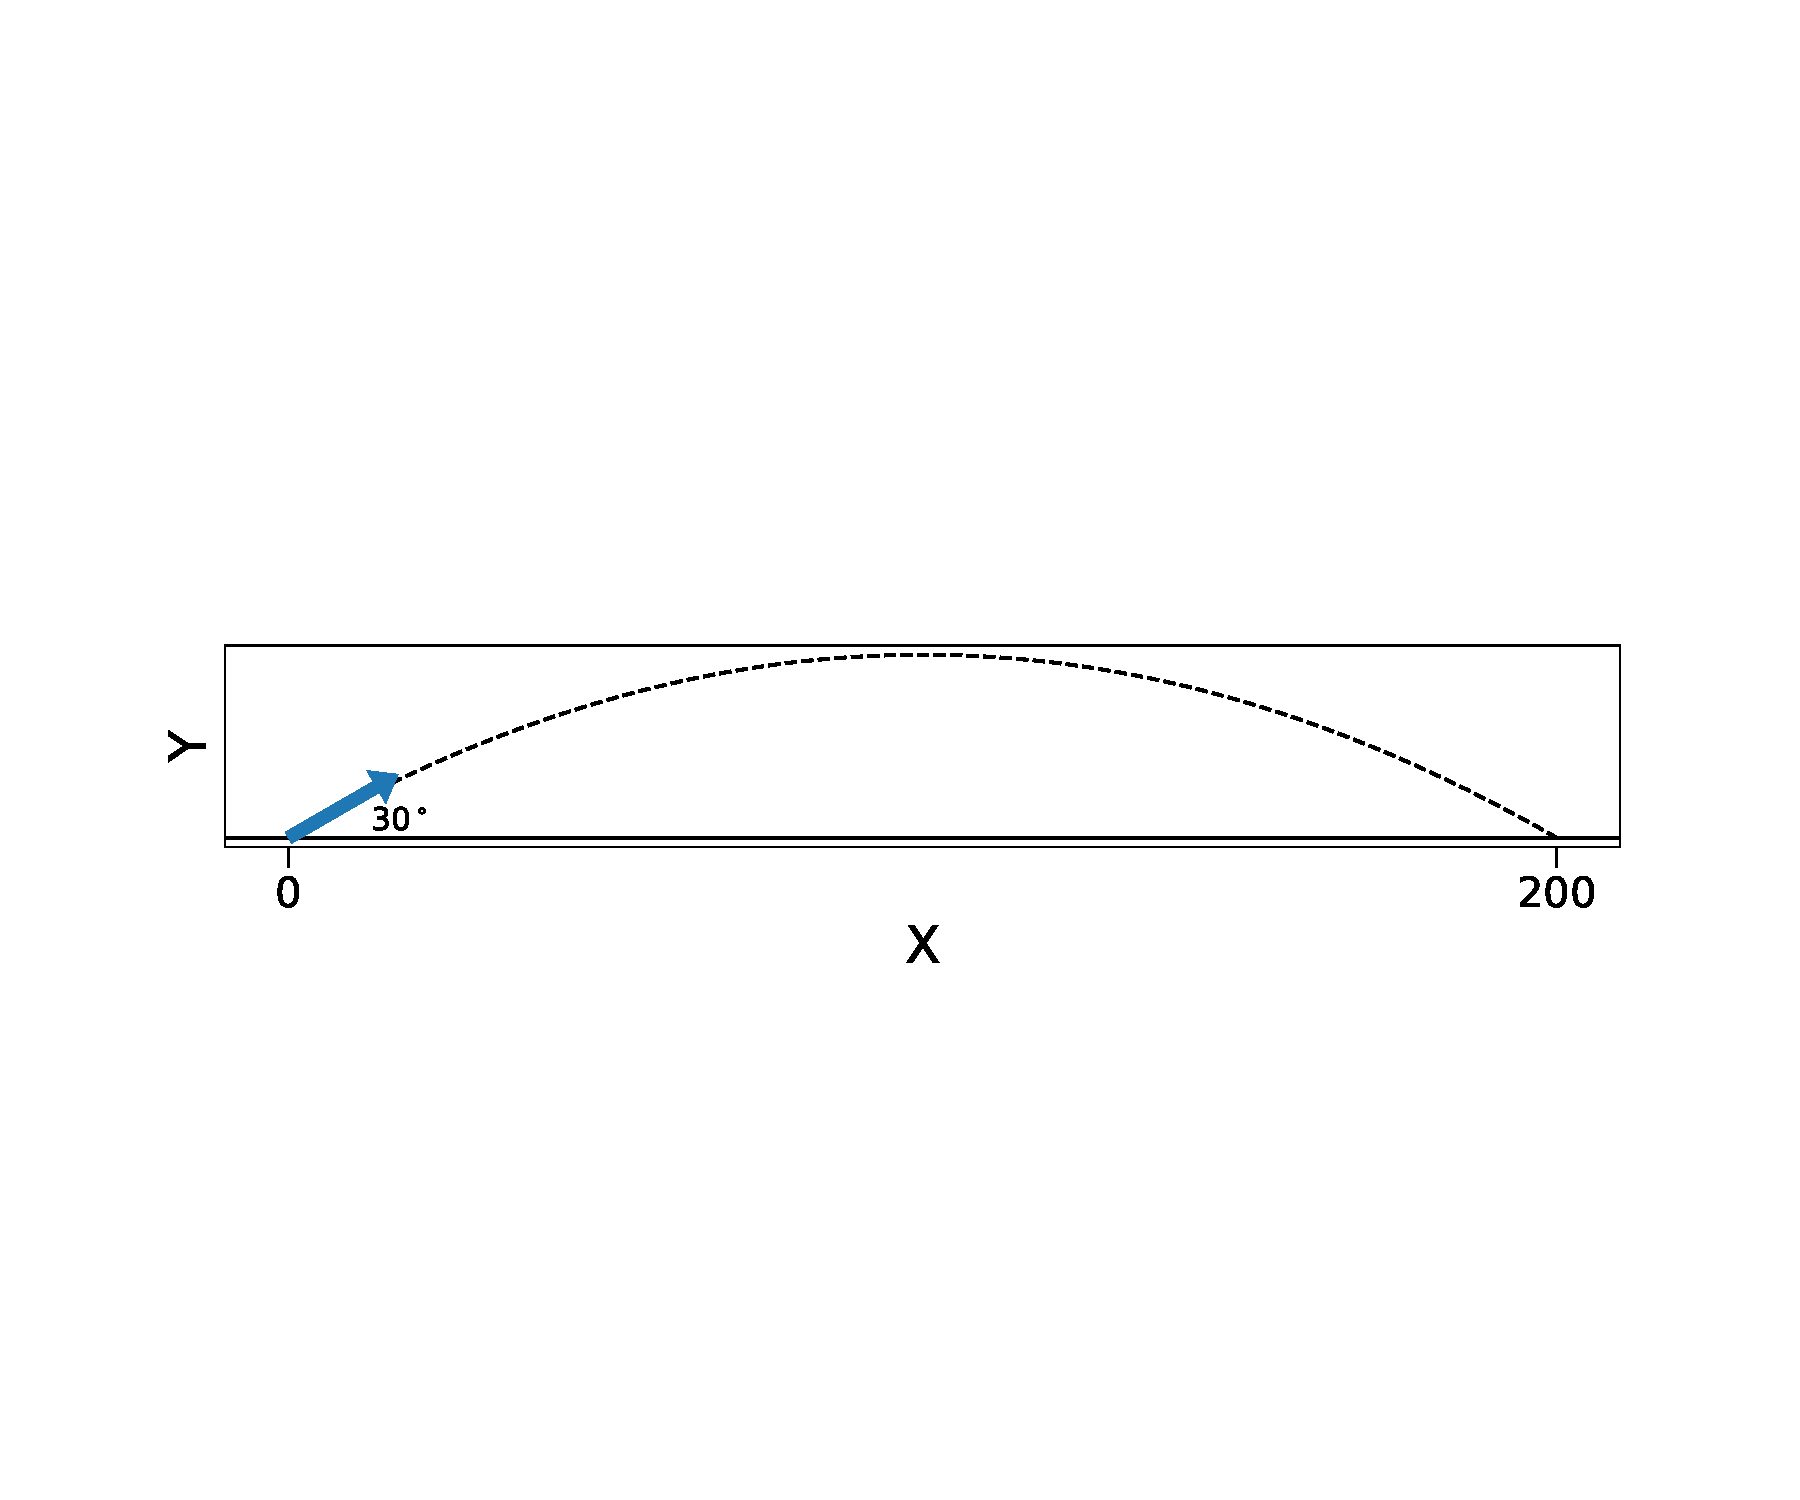
\includegraphics[width=10cm]{projectile_motion}
\end{figure}